\title{Лекция 2\\Базовый язык представления знаний}   
\author[]{Шункевич Д.В.}
\institute[]{Белорусский государственный университет информатики и радиоэлектроники}

\begin{frame}
	\titlepage
\end{frame}

\begin{frame}{\\Содержание лекции}
	\topline
	\justifying
	\begin{itemize}
	\item Основные положения базового языка представления знаний в интеллектуальных системах – SC-кода. 
	\item Алфавит, синтаксис, базовая денотационная семантика SC-кода. 
	\item Синтаксическая и семантическая классификация sc-элементов.
	\end{itemize}
\end{frame}

\begin{frame}{\\Semantic Computer code = SC-code}
	\vspace{10mm}
	\begin{SCn}
	\scnheader{Sc-code} 
	\scnidtf{способ универсального смыслового представления (кодирования) информации в памяти компьютерных систем}
	\vspace{5mm}
	SC-code основан на \textit{теории графов} (синтаксис) и \textit{теории множеств} (семантика), что обеспечивает универсальность и унифицированность (единообразие) представления информации, удобство машинной обработки и восприятия человеком.
	\end{SCn}
\end{frame}

\begin{frame}{\\Сравнение языков представления знаний и информации}
	\vspace{10mm}
	\begin{columns}[T,onlytextwidth]
		\begin{column}{0.5\textwidth}
			\begin{itemize}
				\item[] Двоичное кодирование
				\begin{itemize}
					\item алфавит \{0, 1\}
					\item не удобен для человека
					\item удобен для обработки в компьютере
					\item нельзя понять информацию без контекста
					\item легко реализовать
				\end{itemize}
			\end{itemize}
		\end{column}
		\begin{column}{0.5\textwidth}
			\begin{itemize}
				\item[] SC-code
				\begin{itemize}
					\item базовый алфавит состоит из 5 элементов
					\item удобен для человека
					\item удобен для обработки в компьютере
					\item обладает «осмысленностью»
				\end{itemize}
			\end{itemize}
		\end{column}
	\end{columns}
    \vspace{5mm}
	Переход к "новому качеству" в области информационных технологий будет обусловлен переходом от обработки данных к обработке знаний.
	\\ \textit{From data science to knowledge science}
\end{frame}

\begin{frame}{\\Формы внешнего представления SC-кода}
	\vspace{10mm}
	С помощью SC-кода можно описывать базы знаний, решатели задач и интерфейс интеллектуальной системы. \\ \vspace{5mm}
	SC-code является абстрактным языком, который находится в памяти компьютерной системы. Но его можно визуализировать в различных формах. \\ \vspace{5mm}
	Универсальными формами являются SCg-code (графический), SCn-code(гипертекстовый), SCs-code(текстовый линейный).
\end{frame}

\begin{frame}{\\Формы внешнего представления SC-кода}
	\begin{columns}[T,onlytextwidth]
		\begin{column}{0.4\textwidth}
				\begin{SCn}
					\scnheader{SCs}
					\scnidtf{Semantic Code string}
					\scnidtf{Язык линейного представления знаний}
				
					\scnheader{SCn}
					\scnidtf{Semantic Code natural}
					\scnidtf{Язык структурированного представления знаний}
					
					\scnheader{SCg}
					\scnidtf{Semantic Code graphic}
					\scnidtf{Язык графического представления знаний}
				\end{SCn}
		\end{column}
		\begin{column}{0.5\textwidth}
			\vspace{10mm}
			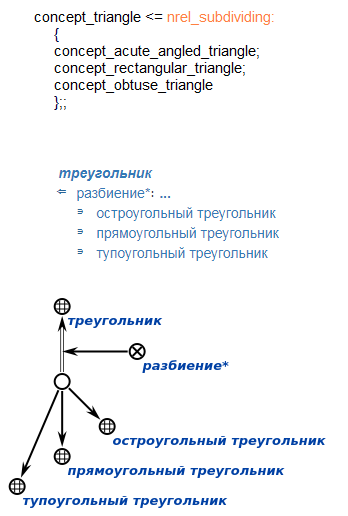
\includegraphics[width=50mm]{./part1/pictures/ostis-basics-1.png}
		\end{column}
	\end{columns}
\end{frame}

\begin{frame}{\\Данные, информация, знания}
	\vspace{10mm}
	\begin{SCn}
	\scnheader{данные}
	\scnidtf{набор значений (фактов, цифр и т.д.)}

	\scnheader{информация}
	\scnidtf{любые сведения об окружающем мире независимо от формы их представления}

	\scnheader{знания}
	\scnidtf{семантически и синтаксически целостная информация}
	\end{SCn}
\end{frame}

\begin{frame}{\\Семантические сети}
	\vspace{10mm}
	\begin{SCn}
	\scnheader{семантическая сеть}
	\scnidtf{граф, вершины которого являются знаками некоторых сущностей, а дуги (ребра) – знаками связей между этими сущностями}
	\scnheader{семантика знака}
	\scnidtf{отношение между знаком и сущностью (значением знака, денотатом), которую он обозначает}
	\begin{center}
		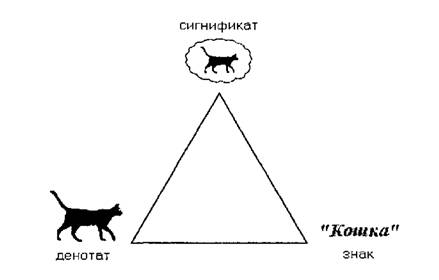
\includegraphics[width=60mm]{./part1/pictures/sc-code-cat.jpg}
	\end{center}
	\end{SCn}
\end{frame}

\begin{frame}{\\Семантические сети}
	\vspace{10mm}
		\begin{center}
			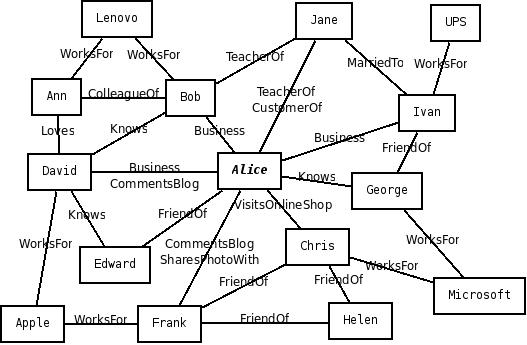
\includegraphics[width=90mm]{./part1/pictures/sc-code-web.jpg}
		\end{center}
\end{frame}

\begin{frame}{\\Алфавит SCg-code}
	
\end{frame}









